\chapter{THC-RCCSD method
\label{sec:THC-RCCSD}}

\section{Introduction}
In this section we present the first application of our tensor structured 
coupled cluster theory. We start with the RCCSD method, where both two body 
interaction part of the Hamiltonian and ${}^2T$ amplitudes have THC structure. 
This combination of decompositions results in a procedure with quartic cost in 
the basis size $N$ and the ranks of THC approximation.

THC approximation is applied in two different ways. First, a decomposition 
of a (constant) two-electron interaction tensor in the Hamiltonian is 
calculated at the beginning of the CC procedure. Second, the factors in the 
THC decomposition of ${}^2T$ are initialized with small random numbers, 
and then updated according to the modified CC iteration we derived in 
Eqn.~\ref{fig:cc_thc_als}. Note that ${}^2T$ is never built as 
a 4-index tensor, but rather optimized in a decomposed form.

Diagrammatically, our choice of decompositions in THC-RCCSD can be summarized 
as:
%
\begin{equation}
%\vcenter{\hbox{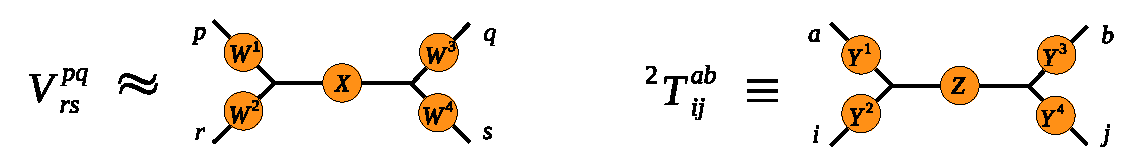
\includegraphics[width=0.95\textwidth]{figures/rccsd_thc_def}}.
\label{fig:rccsd_thc_def}
\end{equation}
%
As diagrams show, two electron interaction is decomposed in Mulliken order, as 
well as two body excitation amplitudes. To study the properties of THC-RCCSD 
we calculated energies of a set of small to medium size weakly 
correlated molecules.

In our setup the decomposition of the electron interaction tensor was 
calculated with a two step method, as described in 
Ref.~\cite{schutski2017tensor} First, partial singular value decomposition of 
the integrals in AO basis was calculated. We retained $r_{V}$ singular values 
and vectors. For larger systems, listed in Tab.~\ref{Tab:Energies}, RI 
decomposed two electron integrals were used in place of singular 
vectors. Next, a CP decomposition of rank $r_{V}$ of the resulting 
left and right singular vectors (arranged as three index tensors of size $N 
\times N \times r_{V}$) was calculated with ALS. The iterative least squares 
procedure was stopped when the ratio of the objective function $f$ to the 
square of the Frobenius norm of the original tensor dropped below $10^{-14}$, or 
a limit of 1000 iterations was reached.

In the subsequent coupled cluster calculations we chose the rank of THC 
decomposition of ${}^2T$ amplitudes ($r_{T}$) to be equal to the rank 
used in approximating integrals, e.g. $r_{T} = r_{V}$. 
The CC iterations were stopped either after the energy was converged to within 
$10^{-9}$ Hartree or a limit of 250 iterations 
was reached. All calculations used the cc-pVDZ basis from EMSL
database,\cite{schuchardt2007basis} and the corresponding cc-pVDZ-RI
was used in the RI approximation. The threshold for pseudoinverses was set to 
$10^{-10}$.

\section{Accuracy of THC for two electron integral approximation}
The accuracy of the THC decomposition of the two-electron integrals governs the
accuracy of the energy in subsequent calculations. Thus, it is important to 
check the dependence of the error in the decomposition of
two-electron integrals on THC rank. Figure~\ref{fig:thc_err_mo_3systems} plots 
this error in a double logarithmic scale for three small molecules. Once again, 
we note that the decomposition is computationally useful if the rank 
$r_\mathrm{V}$ is close to the number of basis functions $N$.  As the figure 
shows, the error in the two-electron integrals decreases exponentially with
respect to THC rank.  We found that this trend holds for every system
tested. Further, there is no significant difference whether the two-electron 
integrals are decomposed in the atomic orbital or molecular orbital basis, as 
is demonstrated in Figure~\ref{fig:thc_err_ao_vs_mo}.

%
\begin{figure}[tb]
%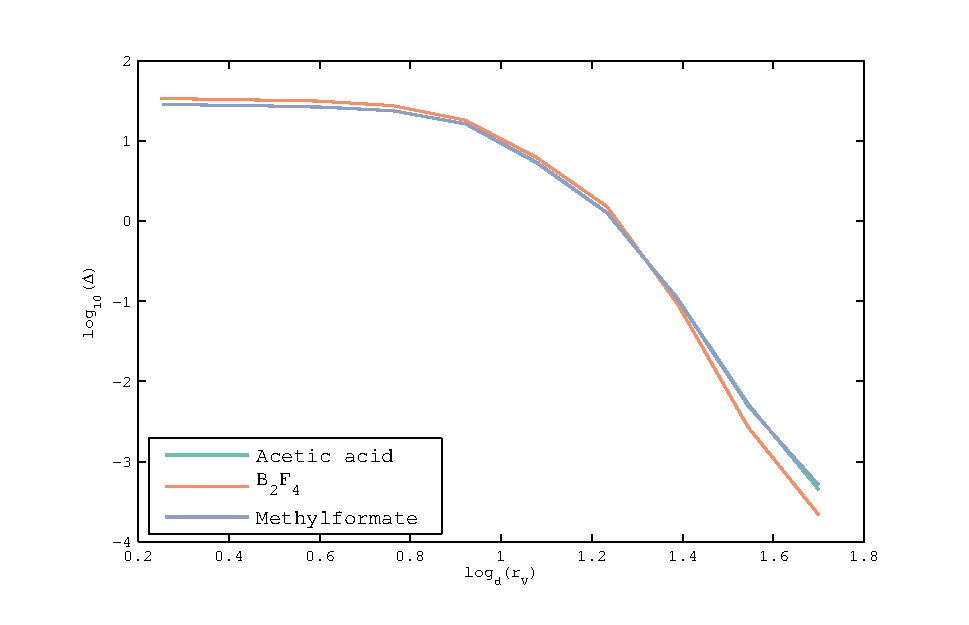
\includegraphics[width=\columnwidth]{figures/thc_err_mo_3systems}
\caption{Frobenius norm of error in decomposed two electron integrals.
\label{fig:thc_err_mo_3systems}}
\end{figure}
%
\begin{figure}[tb]
%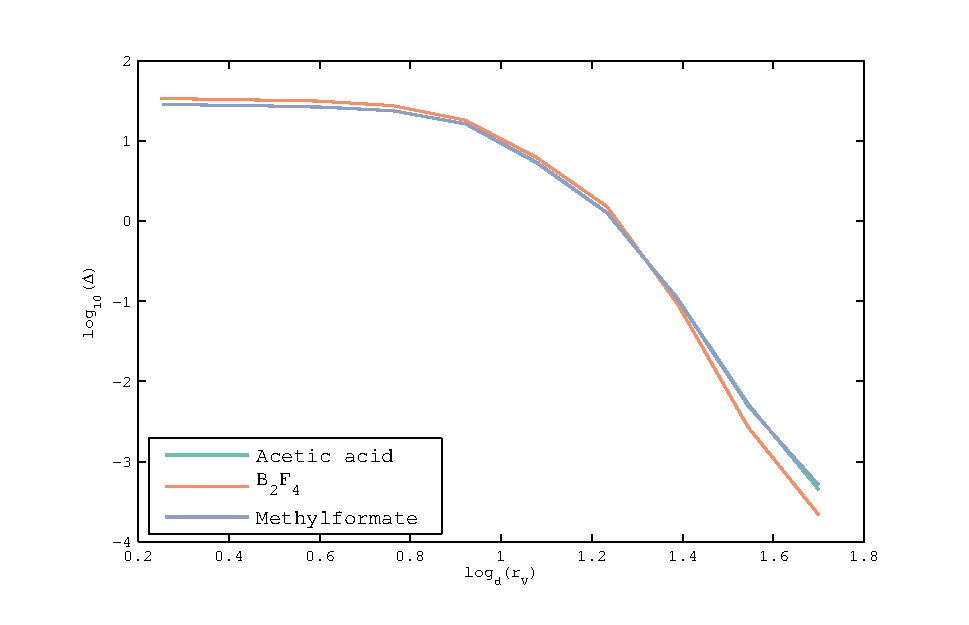
\includegraphics[width=\columnwidth]{figures/thc_err_mo_3systems}
\caption{Frobenius norm of error in decomposed two electron integrals of Acetic 
Acid in atomic and molecular orbital bases.
\label{fig:thc_err_ao_vs_mo}}
\end{figure}
%

To see how these errors of the THC approximation of two-electron 
integrals influence the accuracy of subsequent energies, we checked 
the error in the second-order M{\o}ller-Plesset (MP2) correlation
energy, as shown in Fig.~\ref{fig:mp2_err_ao_full}.  The combination
of MP2 and THC was first proposed by Hohenstein \emph{et
al}.\cite{hohenstein_thc2} and scales as $O(N^4)$.  The way these authors were 
calculating THC decomposition, however, was quite different from ours.
As we found, the error in the MP2 correlation energy follows the trend seen in 
the decomposition of the two-electron integrals (see 
Fig.~\ref{fig:mp2_err_ao_full}). Results within $0.1~mH$
of the exact MP2 correlation energy are already achieved with
$r_\mathrm{V} \sim N^{1.2} - N^{1.4}$.
We expect that the THC would work even better for larger and more extended 
systems as the two-electron integrals become sparser and a lower rank 
decomposition would correspondingly become more accurate.
%
\begin{figure}[tb]
%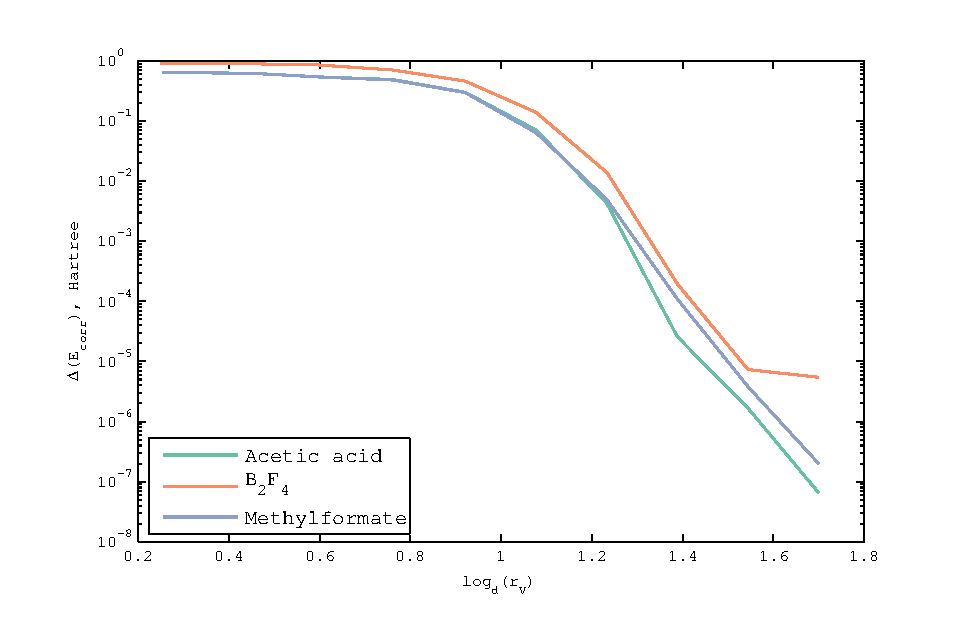
\includegraphics[width=\columnwidth]{figures/mp2_err_ao_full}
\caption{Absolute error in the MP2 correlation energy.
\label{fig:mp2_err_ao_full}}
\end{figure}
%
\section{Accuracy of THC-RCCSD}
We are up to demonstrate the accuracy the THC-decomposed RCCSD
method. Note that we set the rank in THC of amplitudes to equal the rank 
used in the decomposition of two electron integrals. The error in the RCCSD 
correlation energy has a non-monotonic dependence on THC rank, but follows the 
same basic trends as seen in Fig.~\ref{fig:thc_err_mo_3systems} and
Fig.~\ref{fig:mp2_err_ao_full}. Similarly to the case of MP2, errors on 
the order of $0.1~mH$ are achieved with $r_\mathrm{T} = r_\mathrm{V} \sim 
N^{1.2} - N^{1.4}$.
%
\begin{figure}[tb]
%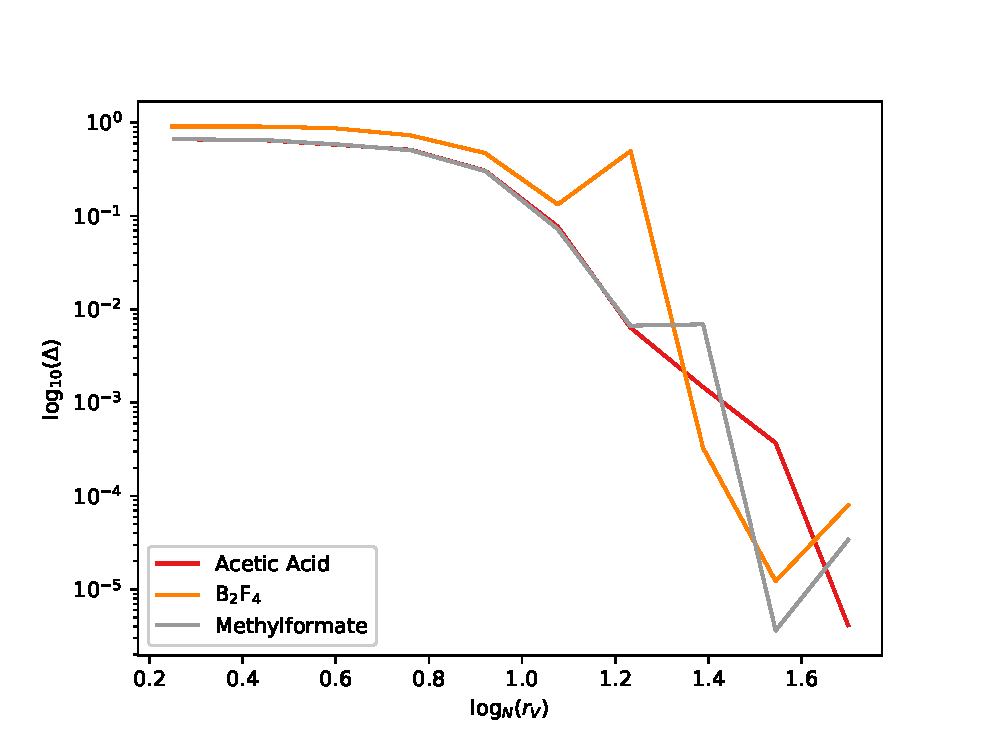
\includegraphics[width=\columnwidth]{figures/cc_err_ao_full}
\caption{Absolute error in the RCCSD correlation energy.
\label{fig:cc_err_ao_full}}
\end{figure}
%
It is interesting to estimate what part of the error in energy can be
attributed to the approximation of the Hamiltonian only. For this reason we 
calculated the correlation energy with converged THC-RCCSD amplitudes but exact
two-electron integrals.  As Fig.~\ref{fig:cc_err_ao_full_amps_only}
shows, using the exact two-electron integrals substantially decreases the error 
in energy, which later motivated us to look for better ways of decomposing the 
two electron integrals. The non-monotonic behavior of the error (compared to 
MP2) can be attributed to the nonlinear nature of the coupled cluster 
equations, which can be quite sensitive to changes in the parameters of the 
Hamiltonian.
%
\begin{figure}[tb]
%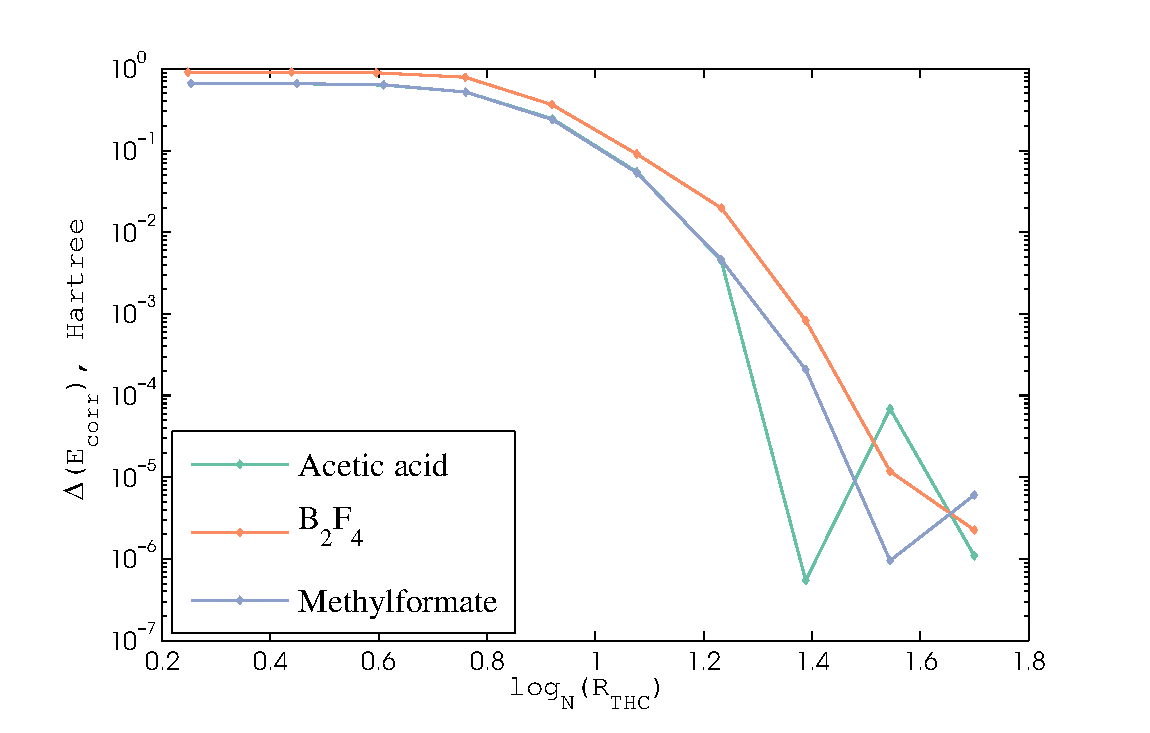
\includegraphics[width=\columnwidth]{figures/cc_err_ao_full_amps_only}
\caption{Absolute error in the RCCSD correlation energy with exact two
electron integrals.
\label{fig:cc_err_ao_full_amps_only}}
\end{figure}
%
\section{Convergence of THC-RCCSD}
Finally, let us discuss the convergence of the THC-RCCSD. In this 
work we used a simple iterative algorithm to solve THC-RCCSD equations, and 
stoped iterations when a specified difference in energy between subsequent 
steps was reached. We found that the convergence of the resulting algorithm is 
highly dependent on the rank chosen for the THC approximation. 
Figure~\ref{fig:cc_thc_convergence} shows the 
number of iterations the algoritm had to take to reach $\theta = 1\cdot 10^{6} 
H$ difference in energy.
%
\begin{figure}[tb]
%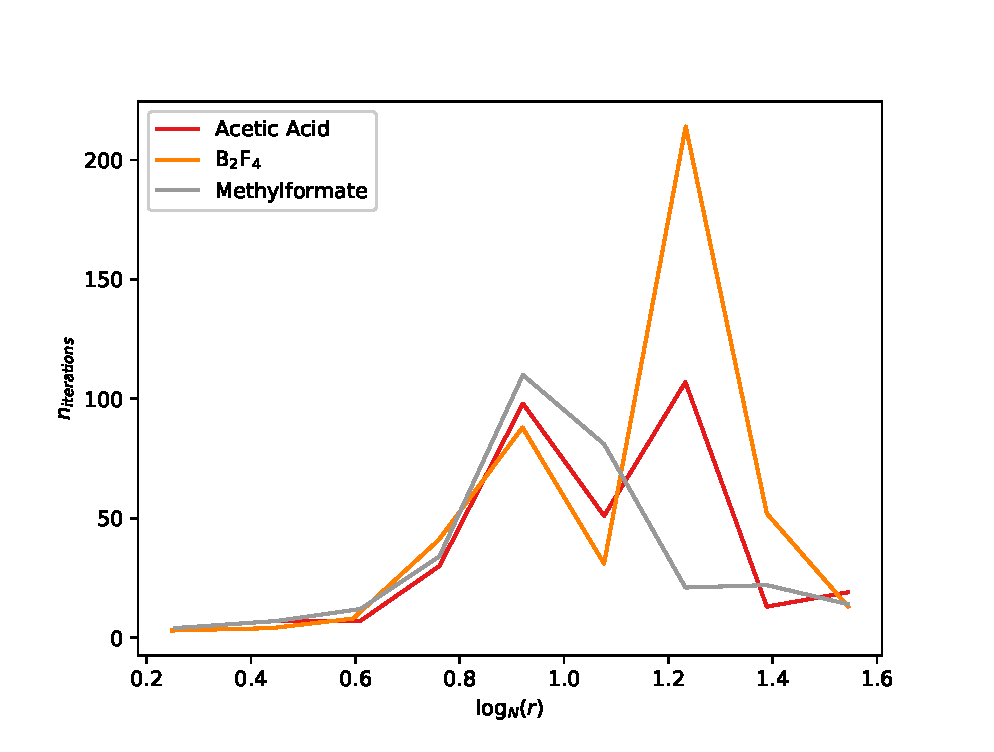
\includegraphics[width=\columnwidth]{figures/niter_vs_logr}
\caption{Number of iterations of THC-RCCSD to reach $1 \cdot 10^{-6} H$ 
difference in energy}
\label{fig:cc_thc_convergence}
\end{figure}
%
For small as well as larger THC ranks the convergence of THC-RCCSD is 
comparable 
or better than regular RCCSD (if simple iterations were used). In the 
intermediate regime, however, the algorithm may need
a large number of iterations to converge. We note that the convergence in this 
regime significantly depended on the choice of initial parameters and several 
random trials needed to find good ones. 
We provide the following tentative explanation to the observed behavior. As 
THC-RCCSD in our formulation
is a sum of two iterative algorithms, merely, an ALS step and a CC iteration, 
there is a competition between 
updates each of these parts is generating. In case of small ranks the update 
should be mostly determined by ALS, as ${}^{2}T$ amplitudes are poorly 
approximated with any set of parameters $Y$. In 
contrast, with larger ranks mostly CC equations govern the update, because 
${}^2T$ is well approximated
 at each step. We admit, however, that the means to control convergence of our 
hybrid algorithms 
need a further study. All later numerical experiments were done in a regime 
where THC-RCCSD performs
similarly to regular RCCSD, e. g. where THC ranks are relatively large. 


\subsubsection{{Larger systems}
\label{sec:larger_systems}}

Having seen how the THC-RCCSD method performs for various THC
decomposition ranks, we tested the method on a set of small and
medium-sized molecules introduced in previous work on
THC.\cite{hohenstein_thc3} Technical details of the calculations,
including molecular geometries and reference energies, are provided in
the supplementary materials.  We chose the ranks of the THC
decomposition of the amplitudes and integrals to be similar to the
number of functions $N_\mathrm{RI}$ in the basis used in the RI
approximation. {\color{blue} Energies, differences with respect to regular 
Coupled Cluster,
the number of CC iterations and norm of final residuals are presented in 
Table~\ref{Tab:Energies}}.  We
used RI for all these calculations.
%

\begin{center}
\begin{table}[h]
\caption{CCSD correlation energies ($E_c$), errors in
correlation energies ($\Delta E_c$), number of THC-RCCSD iterations 
($n_{iter}$) 
and the norm of doubles residuals ($|{}^2R_{ij}^{ab}|$) for several small 
molecules.
\label{Tab:Energies}}
\begin{tabular}{lccccccc}
& & \multicolumn{2}{c}{$\Delta E_c (mH)$} & \multicolumn{2}{c}{$n_{iter}$} & 
\multicolumn{2}{c}{$|{}^2R_{ij}^{ab}|$}\\
\cline{3-4} \cline{5-6} \cline{7-8} System & $E_c (mH)$ & $N_\mathrm{RI}$ &
$1.5 \, N_\mathrm{RI}$ & $N_\mathrm{RI}$ &
$1.5 \, N_\mathrm{RI}$ & $N_\mathrm{RI}$ &
$1.5 \, N_\mathrm{RI}$\\
\hline
Acetic acid & -666.510 & -0.579 & -0.453 & 50 & 31 & 0.041 & 0.033 \\
Aniline & -997.193 & -1.177 & -0.471 & 111 & 64 & 0.051 & 0.032 \\
Diboron tetrafluoride & -909.944 & -0.702 & -0.716 & 15 & 17 & 0.053 & 0.034\\
Benzene & -823.101 & -0.985 & -0.450 & 111 & 62 & 0.048 & 0.030\\
Butadiene & -581.340 & -0.710 & -0.274 & 41 & 42 & 0.041 & 0.025\\
Cyclobutane & -621.099 & -0.895 & -0.290 & 77 & 50 & 0.039 & 0.028\\
Dimethylsulfoxide & -661.870 & 0.195 & -0.624 & 287 & 39 & 0.056 & 0.025\\
Furan & -736.463 & -0.865 & -0.454 & 73 & 50 & 0.046 & 0.033\\
Isobutane & -652.505 & -0.876 & -0.263 & 78 & 49 & 0.035 & 0.025\\
Methylformate & -666.805 & -0.586 & -0.455 & 62 & 35 & 0.042 & 0.032\\
Methylnitrite & -708.990 & -0.476 & -0.492 & 68 & 47 & 0.047 & 0.033\\
Phenol & -1005.727 & -0.887 & -0.514 & 120 & 59 & 0.051 & 0.032\\
Pyridine & -842.453 & -1.045 & -0.475 & 104 & 61 & 0.047 & 0.032\\
Pyrrole & -727.051 & -0.855 & -0.407 & 84 & 52 & 0.045 & 0.032\\
Thiophene & -695.593 & -1.013 & -0.657 & 97 & 52 & 0.039 & 0.032\\
Toluene & -980.030 & -1.270 & -0.461 & & & &\\
\hline
MUE\footnote{mean unsigned error} & & 0.820 & 0.466 & & & &\\
Max\footnote{maximum unsigned error} & & 1.270 & 0.716 & & & &\\
RMS\footnote{root-mean-square error} & & 0.861 & 0.482 & & & &\\
\end{tabular}
\end{table}

\end{center}
%
{\color{blue} Let us highlight some results in Table~\ref{Tab:Energies}.
As THC-RCCSD is an approximation to regular CC equations,
the full residuals may not be zero, because the number of CC equations is 
usually much larger that the number of parameters of THC-RCCSD. 
An interesting observation is that despite the norm of 
doubles residuals is not negligible in THC-RCCSD, the error in energy 
is quite low. This contrasts with conventional CC, where the 
difference of energy with the final value during iterations 
is proportional to the norm of the residuals. Also, we observed
a generically faster convergence of energy in THC-RCCSD for larger ranks.
}

We note that our results are on par with calculations of
Hohenstein \emph{et al.},\cite{hohenstein_thc3} but similar errors are achieved 
with
ranks which are roughly half as large.  Presumably this is because in
previous work most of the factors in the THC decomposition of the
amplitudes were kept fixed (except $Z$), whereas our scheme optimizes
all factors, therefore providing greater flexibility and reaching the
exact decomposition quicker. 
{\color{blue} It should be noted that most of the time in our 
calculations was spent on the decomposition of the Hamiltonian rather
than on the solution of approximated CC equations. 
Quadrature based methods for building THC, such as the ones described in
Refs.~\cite{hohenstein_thc1} and~\cite{parrish2013discrete}, may be much
faster than iterative approaches, and reach the same accuracy as ALS-based 
THC with about 3x more factors.\cite{parrish2013discrete}
Hence we recommend a hybrid scheme for future developments of THC based methods:
one may build THC of the Hamiltonian with real space quadratures, in a way shown
in Ref.~\cite{hohenstein_thc2}, and later solve for the factors of doubles in 
the 
way we developed}. Again, we emphasize that the proposed
scheme is not limited to THC, and can be applied to many other
decompositions, which is the topic of ongoing investigation.
